% Options for packages loaded elsewhere
\PassOptionsToPackage{unicode}{hyperref}
\PassOptionsToPackage{hyphens}{url}
%
\documentclass[
  12 pt,
  a4paper,
]{article}
\usepackage{amsmath,amssymb}
\usepackage{setspace}
\usepackage{iftex}
\ifPDFTeX
  \usepackage[T1]{fontenc}
  \usepackage[utf8]{inputenc}
  \usepackage{textcomp} % provide euro and other symbols
\else % if luatex or xetex
  \usepackage{unicode-math} % this also loads fontspec
  \defaultfontfeatures{Scale=MatchLowercase}
  \defaultfontfeatures[\rmfamily]{Ligatures=TeX,Scale=1}
\fi
\usepackage{lmodern}
\ifPDFTeX\else
  % xetex/luatex font selection
  \setmainfont[]{Times New Roman}
\fi
% Use upquote if available, for straight quotes in verbatim environments
\IfFileExists{upquote.sty}{\usepackage{upquote}}{}
\IfFileExists{microtype.sty}{% use microtype if available
  \usepackage[]{microtype}
  \UseMicrotypeSet[protrusion]{basicmath} % disable protrusion for tt fonts
}{}
\makeatletter
\@ifundefined{KOMAClassName}{% if non-KOMA class
  \IfFileExists{parskip.sty}{%
    \usepackage{parskip}
  }{% else
    \setlength{\parindent}{0pt}
    \setlength{\parskip}{6pt plus 2pt minus 1pt}}
}{% if KOMA class
  \KOMAoptions{parskip=half}}
\makeatother
\usepackage{xcolor}
\usepackage[margin=1in]{geometry}
\usepackage{color}
\usepackage{fancyvrb}
\newcommand{\VerbBar}{|}
\newcommand{\VERB}{\Verb[commandchars=\\\{\}]}
\DefineVerbatimEnvironment{Highlighting}{Verbatim}{commandchars=\\\{\}}
% Add ',fontsize=\small' for more characters per line
\usepackage{framed}
\definecolor{shadecolor}{RGB}{248,248,248}
\newenvironment{Shaded}{\begin{snugshade}}{\end{snugshade}}
\newcommand{\AlertTok}[1]{\textcolor[rgb]{0.94,0.16,0.16}{#1}}
\newcommand{\AnnotationTok}[1]{\textcolor[rgb]{0.56,0.35,0.01}{\textbf{\textit{#1}}}}
\newcommand{\AttributeTok}[1]{\textcolor[rgb]{0.13,0.29,0.53}{#1}}
\newcommand{\BaseNTok}[1]{\textcolor[rgb]{0.00,0.00,0.81}{#1}}
\newcommand{\BuiltInTok}[1]{#1}
\newcommand{\CharTok}[1]{\textcolor[rgb]{0.31,0.60,0.02}{#1}}
\newcommand{\CommentTok}[1]{\textcolor[rgb]{0.56,0.35,0.01}{\textit{#1}}}
\newcommand{\CommentVarTok}[1]{\textcolor[rgb]{0.56,0.35,0.01}{\textbf{\textit{#1}}}}
\newcommand{\ConstantTok}[1]{\textcolor[rgb]{0.56,0.35,0.01}{#1}}
\newcommand{\ControlFlowTok}[1]{\textcolor[rgb]{0.13,0.29,0.53}{\textbf{#1}}}
\newcommand{\DataTypeTok}[1]{\textcolor[rgb]{0.13,0.29,0.53}{#1}}
\newcommand{\DecValTok}[1]{\textcolor[rgb]{0.00,0.00,0.81}{#1}}
\newcommand{\DocumentationTok}[1]{\textcolor[rgb]{0.56,0.35,0.01}{\textbf{\textit{#1}}}}
\newcommand{\ErrorTok}[1]{\textcolor[rgb]{0.64,0.00,0.00}{\textbf{#1}}}
\newcommand{\ExtensionTok}[1]{#1}
\newcommand{\FloatTok}[1]{\textcolor[rgb]{0.00,0.00,0.81}{#1}}
\newcommand{\FunctionTok}[1]{\textcolor[rgb]{0.13,0.29,0.53}{\textbf{#1}}}
\newcommand{\ImportTok}[1]{#1}
\newcommand{\InformationTok}[1]{\textcolor[rgb]{0.56,0.35,0.01}{\textbf{\textit{#1}}}}
\newcommand{\KeywordTok}[1]{\textcolor[rgb]{0.13,0.29,0.53}{\textbf{#1}}}
\newcommand{\NormalTok}[1]{#1}
\newcommand{\OperatorTok}[1]{\textcolor[rgb]{0.81,0.36,0.00}{\textbf{#1}}}
\newcommand{\OtherTok}[1]{\textcolor[rgb]{0.56,0.35,0.01}{#1}}
\newcommand{\PreprocessorTok}[1]{\textcolor[rgb]{0.56,0.35,0.01}{\textit{#1}}}
\newcommand{\RegionMarkerTok}[1]{#1}
\newcommand{\SpecialCharTok}[1]{\textcolor[rgb]{0.81,0.36,0.00}{\textbf{#1}}}
\newcommand{\SpecialStringTok}[1]{\textcolor[rgb]{0.31,0.60,0.02}{#1}}
\newcommand{\StringTok}[1]{\textcolor[rgb]{0.31,0.60,0.02}{#1}}
\newcommand{\VariableTok}[1]{\textcolor[rgb]{0.00,0.00,0.00}{#1}}
\newcommand{\VerbatimStringTok}[1]{\textcolor[rgb]{0.31,0.60,0.02}{#1}}
\newcommand{\WarningTok}[1]{\textcolor[rgb]{0.56,0.35,0.01}{\textbf{\textit{#1}}}}
\usepackage{graphicx}
\makeatletter
\def\maxwidth{\ifdim\Gin@nat@width>\linewidth\linewidth\else\Gin@nat@width\fi}
\def\maxheight{\ifdim\Gin@nat@height>\textheight\textheight\else\Gin@nat@height\fi}
\makeatother
% Scale images if necessary, so that they will not overflow the page
% margins by default, and it is still possible to overwrite the defaults
% using explicit options in \includegraphics[width, height, ...]{}
\setkeys{Gin}{width=\maxwidth,height=\maxheight,keepaspectratio}
% Set default figure placement to htbp
\makeatletter
\def\fps@figure{htbp}
\makeatother
\setlength{\emergencystretch}{3em} % prevent overfull lines
\providecommand{\tightlist}{%
  \setlength{\itemsep}{0pt}\setlength{\parskip}{0pt}}
\setcounter{secnumdepth}{-\maxdimen} % remove section numbering
\ifLuaTeX
\usepackage[bidi=basic]{babel}
\else
\usepackage[bidi=default]{babel}
\fi
\babelprovide[main,import]{spanish}
\ifPDFTeX
\else
\babelfont{rm}[]{Times New Roman}
\fi
% get rid of language-specific shorthands (see #6817):
\let\LanguageShortHands\languageshorthands
\def\languageshorthands#1{}
\ifLuaTeX
  \usepackage{selnolig}  % disable illegal ligatures
\fi
\usepackage{bookmark}
\IfFileExists{xurl.sty}{\usepackage{xurl}}{} % add URL line breaks if available
\urlstyle{same}
\hypersetup{
  pdfauthor={tofermos},
  pdflang={es-ES},
  hidelinks,
  pdfcreator={LaTeX via pandoc}}

\title{U2: Activitat de VirtualBox}
\usepackage{etoolbox}
\makeatletter
\providecommand{\subtitle}[1]{% add subtitle to \maketitle
  \apptocmd{\@title}{\par {\large #1 \par}}{}{}
}
\makeatother
\subtitle{Aproximació al VirtualBox i instal·lació mínima d'un Lubuntu}
\author{tofermos}
\date{}

\begin{document}
\maketitle

{
\setcounter{tocdepth}{2}
\tableofcontents
}
\setstretch{1.5}
\newpage
\renewcommand\tablename{Tabla}

\begin{center}\rule{0.5\linewidth}{0.5pt}\end{center}

\section{1 Introducció}\label{introducciuxf3}

Tot i que més avant estudiarem més detingudament la instla·lació i
configuració d'Ubuntu, necessitem fer ara un avanç poder vore entendre,
de manera práctica. què és la virtualització i altres conceptes teòrics.

En aquesta activitat vorem conceptes vistos en la \textbf{Unitat 1}:

\begin{itemize}
\item
  Software de sistema.
\item
  Codi de detecció i correcció de la integritat de les dades.
\end{itemize}

Aprendrem els aspectes més importants del..

\begin{itemize}
\tightlist
\item
  VirtualBox
\end{itemize}

I serà un avanç a la Unitat 5 que tracta la instal·lació del Linux.

\section{2 Instruccions per a
l'activitat}\label{instruccions-per-a-lactivitat}

\begin{enumerate}
\def\labelenumi{\arabic{enumi}.}
\item
  Estudieu la Unitat 1 i Unitat 2.
\item
  Llegiu bé l'\textbf{Apartat 1}. Tot i que tornarem a veure-ho més
  avant.
\item
  A l'\textbf{Apartat 2} s'especifica què heu de fer. Documenteu amb
  captures de pantalla el que aneu fent i guardeu en una carpeta amb el
  nom ``Activitat2''.
\end{enumerate}

*Els apartats següents: \textbf{2.1, 2.2, 2.3} els estudiarem en
la\textbf{UInitat 5}. Ara només cam que els llegiu per entendre quin SO
anem a instal·lar.

\subsection{2.1 Lubuntu/Ubuntu}\label{lubuntuubuntu}

Ubuntu i Lubuntu són diferents versions del mateix sistema operatiu base
(nucli, repositoris i funcionalitats). La principal diferència entre
\textbf{Ubuntu} i \textbf{Lubuntu} es troba en l'entorn
d'\textbf{escriptori} i, conseqüentment, el rendiment. Aquí és on
resideix la diferència:

\begin{itemize}
\item
  \textbf{Ubuntu}: Utilitza l'entorn d'escriptori \textbf{GNOME}, més
  complet, modern i visualment atractiu però més exigent pel que fa a
  l'ús de recursos del sistema (RAM i CPU).
\item
  \textbf{Lubuntu}: Fa servir \textbf{LXQt}, un entorn d'escriptori molt
  més lleuger. Està dissenyat per consumir menys recursos, fent-lo ideal
  per a ordinadors antics i, més encara si, sobre aquests virtualitzem
  com serà el nostra cas a l'aula en el curs 2024-2025.
\end{itemize}

\subsection{2.2 Versions}\label{versions}

Són actualitzacions del sistema operatiu que es publiquen regularment.
Hi ha dues categories principals:

\begin{enumerate}
\def\labelenumi{\arabic{enumi}.}
\tightlist
\item
  \textbf{Versions LTS (Long Term Support)}: Versions amb suport a llarg
  termini (5 anys). Estan dissenyades per ser estables i segures durant
  més temps.
\item
  \textbf{Versions regulars}: Tenen un cicle de vida més curt (9 mesos),
  amb novetats més freqüents però menys estabilitat.
\end{enumerate}

Els escriptoris també tenen versions.

\subsection{2.3 Consultes per terminal}\label{consultes-per-terminal}

Comencem a obrir el Terminal ( \textbf{Alt + T}) i escriure alguna ordre
de Linux\ldots{}

\subsubsection{Quin entorn d'escriptori tenim
?}\label{quin-entorn-descriptori-tenim}

Cal consultar una vairable del sistema. Les estudiarem més avant.

\begin{Shaded}
\begin{Highlighting}[]
\NormalTok{echo $XDG\_CURRENT\_DESKTOP}
\end{Highlighting}
\end{Shaded}

\subsubsection{Quina versió té
l'escriptori?}\label{quina-versiuxf3-tuxe9-lescriptori}

\begin{Shaded}
\begin{Highlighting}[]
\NormalTok{gnoms{-}shell {-}{-}version}
\end{Highlighting}
\end{Shaded}

\subsubsection{Ditribució i versió del
SO?}\label{ditribuciuxf3-i-versiuxf3-del-so}

Fixeu-vos en Description i en Release

\begin{Shaded}
\begin{Highlighting}[]
\NormalTok{lsb\_release {-}a}
\end{Highlighting}
\end{Shaded}

\subsection{Versió del nucli?}\label{versiuxf3-del-nucli}

\begin{Shaded}
\begin{Highlighting}[]
\NormalTok{uname {-}r}
\end{Highlighting}
\end{Shaded}

\begin{quote}
Nota:

La majoria d'ordres (comandaments) de Linux tenen un \textbf{man}ual per
consultar. O una ajuda (help) alternativa.
\end{quote}

Exemple de búsqueda d'ajuda:

\begin{Shaded}
\begin{Highlighting}[]
\NormalTok{man uname}
\end{Highlighting}
\end{Shaded}

\begin{figure}
\centering
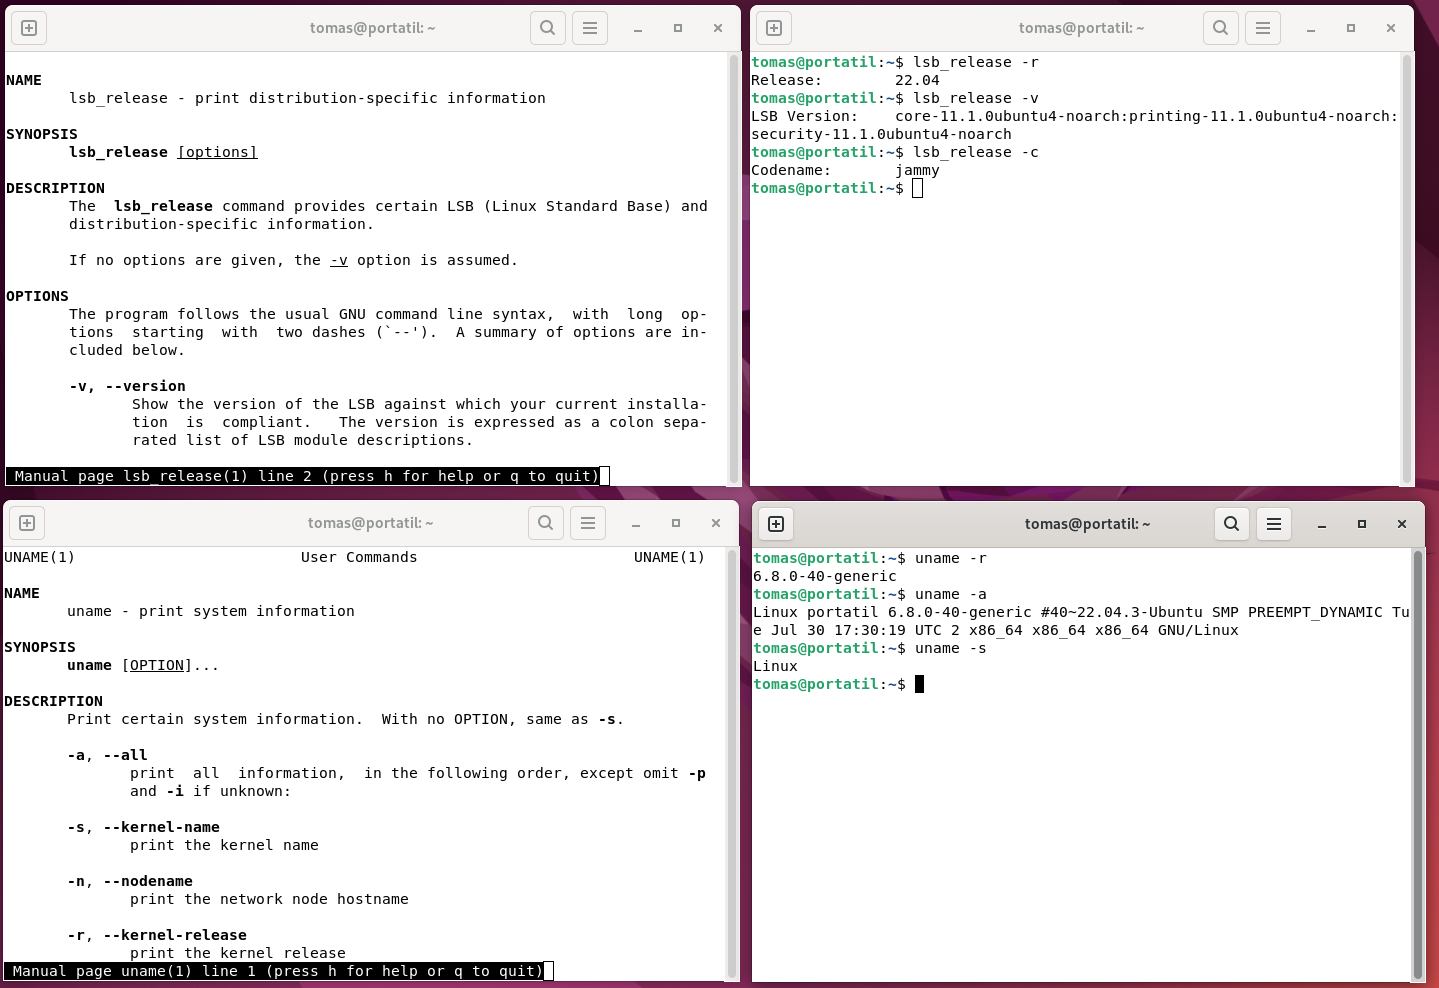
\includegraphics{png/4en1.png}
\caption{Ajuda i execució de 2 ordres al mateix temps}
\end{figure}

\section{3 Activitat}\label{activitat}

\subsection{3.1 Descàrrega i comprovació de la
font}\label{descuxe0rrega-i-comprovaciuxf3-de-la-font}

Descàrrega la ISO de Lubuntu més avançada i fes la comprovació de la
integritat del fitxer descarrega't tal com indica a la web.

\href{https://lubuntu.me/downloads/}{Web Lubuntu}

\begin{figure}
\centering
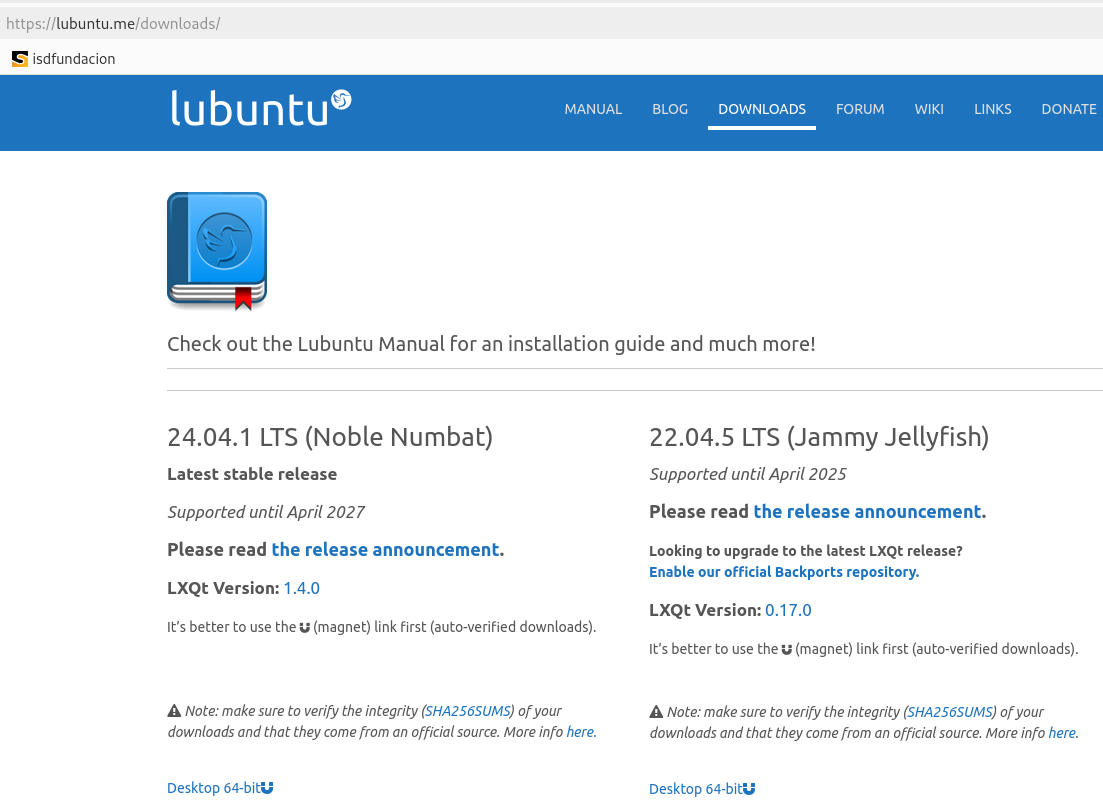
\includegraphics{png/LubuntuWeb.png}
\caption{\emph{Figura1: Web de Lubuntu. Downloads}}
\end{figure}

\subsection{3.2 Comprovar la integritat del
fitxer}\label{comprovar-la-integritat-del-fitxer}

Usarem la \textbf{funció de hash: \emph{sha256}} de Linux per comprovar
que coincidesca amb el codi SHA256 que corresponga; el consultarem en
l'enllaç de la Web.

\begin{figure}
\centering
\includegraphics{png/EnllaçSHA.png}
\caption{Enllaç codi SHA256}
\end{figure}

Estem, per tant fent una comprovació per detectar si hi ha hagut algun
error en la baixada o en la gravació en disc; assegurant la integritat
de les dades.

\begin{quote}
Nota:

Excutar una funció hash, quan ens ho proposa un proveïdor, és una
pràctica recomanable que devem acostumar-nos a fer en descarregar o
copiar software, sobretot si són fitxers de cert tamany.
\end{quote}

Així:

\begin{Shaded}
\begin{Highlighting}[]
\NormalTok{sha256sum lubuntu{-}22.04.5{-}desktop{-}amd64.iso }
\end{Highlighting}
\end{Shaded}

\begin{quote}
Nota: Quan els fitxer sobre passen el \textbf{4Gb} no podràs copiar-los
a un pen-drive formatejar amb FAT32 com solen vidre per defecte. Això
ens passaria amb la ISO de Windows 1x, per exemple. Convé que el
formateges com a NTFS.
\end{quote}

\subsection{3.3 Instal·lació senzilla}\label{installaciuxf3-senzilla}

Ara intentarem fer la instal·lació.

Indicarem on està la ISO (emulem la inserció del Pendrive o DVD)

\begin{figure}
\centering
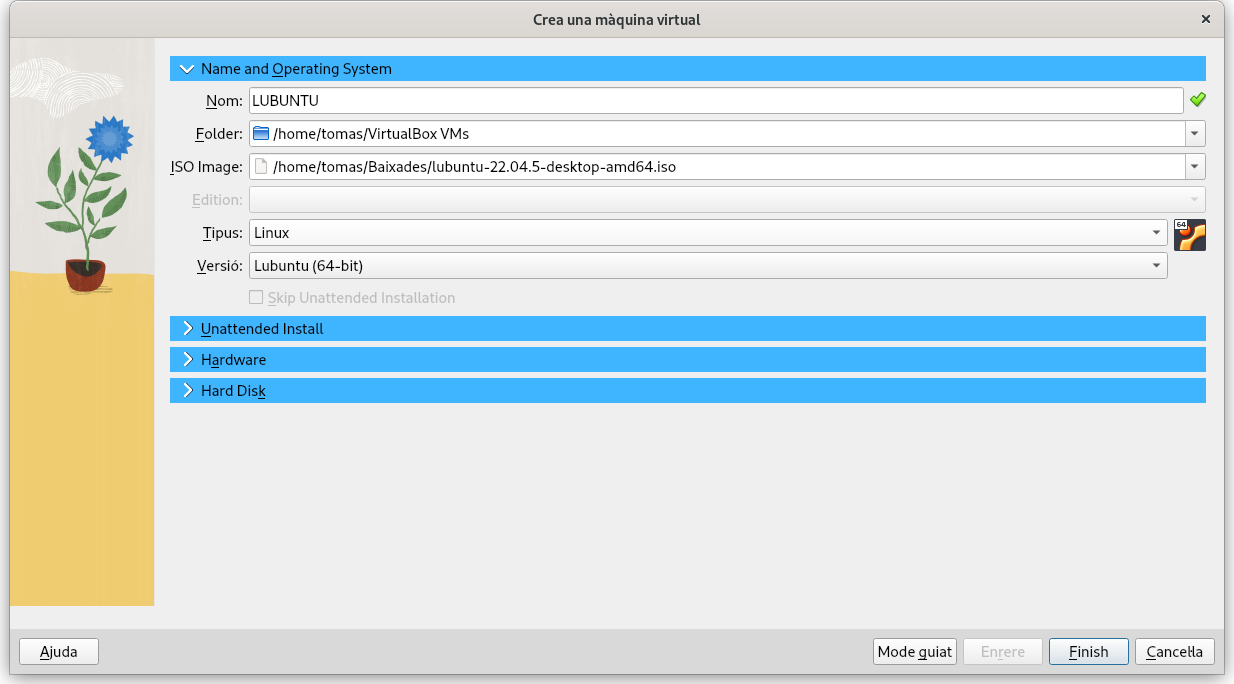
\includegraphics{png/1InstalacioLubuntu.png}
\caption{\emph{Figura 3: Instal·lació pas 1}}
\end{figure}

Indiquem que creem un disco dur nou VDI

\begin{figure}
\centering
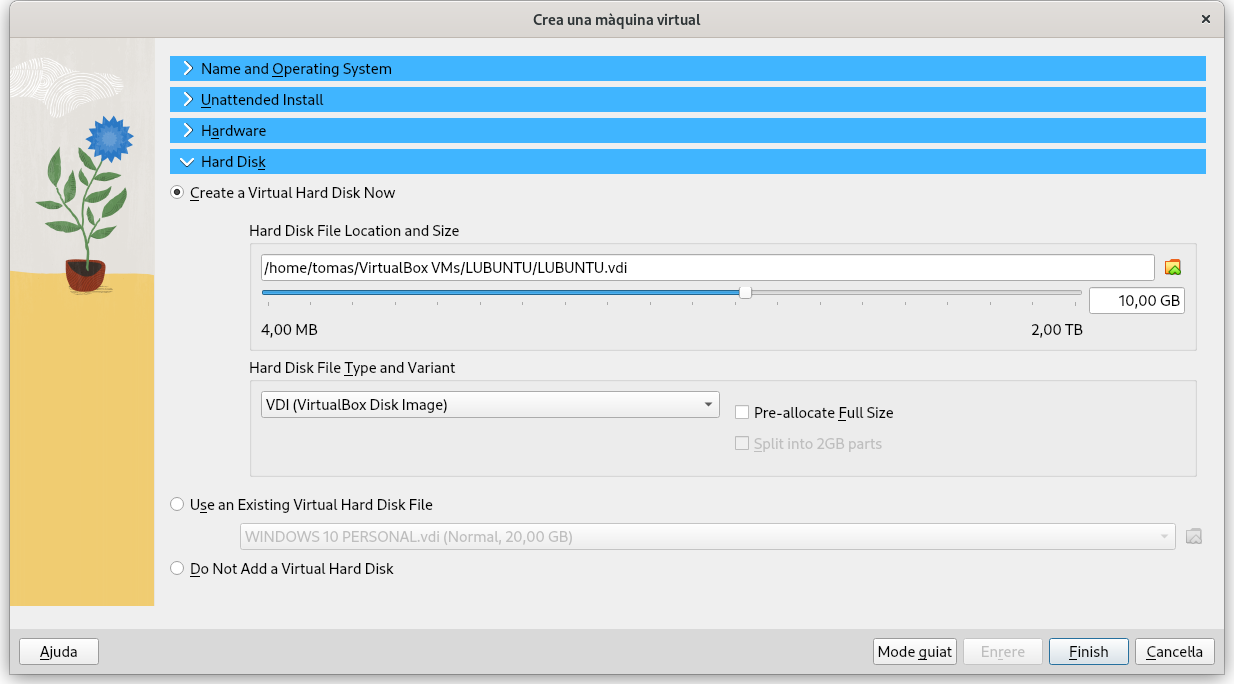
\includegraphics{png/2InstalacioLubuntu.png}
\caption{\emph{Figura 2: Instal·lació pas 2}}
\end{figure}

\subsection{3.4 Configuració}\label{configuraciuxf3}

\begin{figure}
\centering
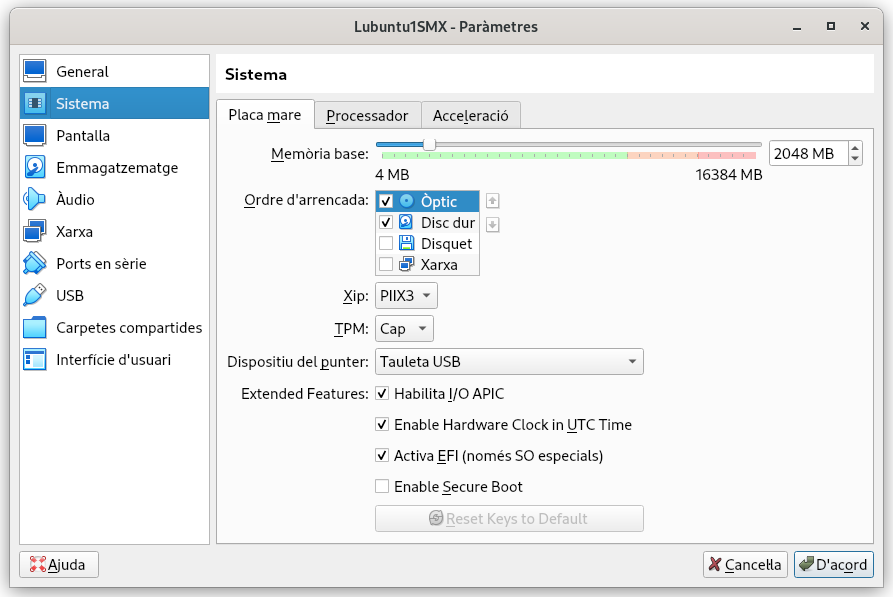
\includegraphics{png/SistemaLubuntu.png}
\caption{\emph{Figura 3: Sistema Lubuntu}}
\end{figure}

\begin{figure}
\centering
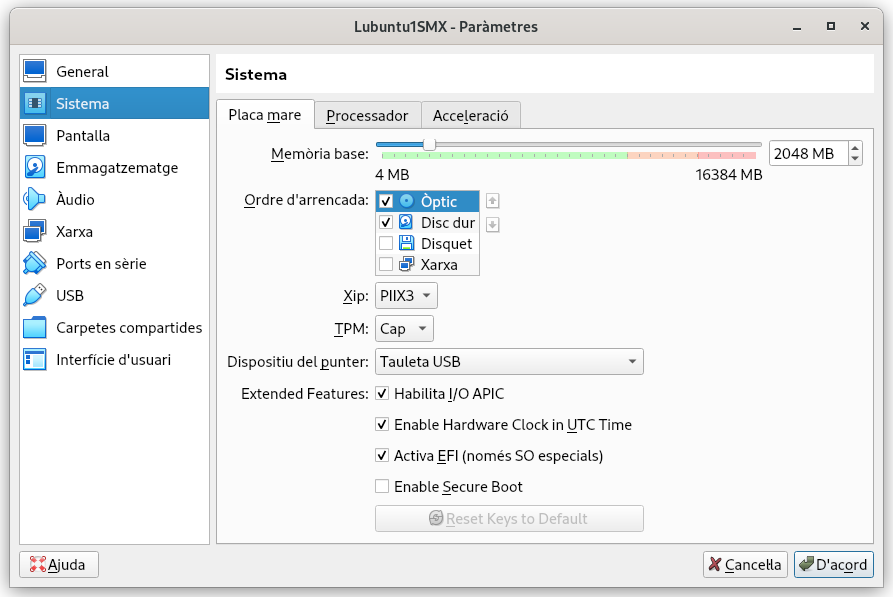
\includegraphics{png/SistemaLubuntu.png}
\caption{\emph{Figura 4: Pantalla Lubuntu}}
\end{figure}

Les opcions que no estiguen explicades a la teoria, les deixarem amb els
seus valors per defecte.

Fixa't en l'usuari i password per defecte que et crea. Si fas algun
canvi, anota-te'l.

\end{document}
